% Created by tikzDevice version 0.8.1 on 2015-11-17 12:44:46
% !TEX encoding = UTF-8 Unicode
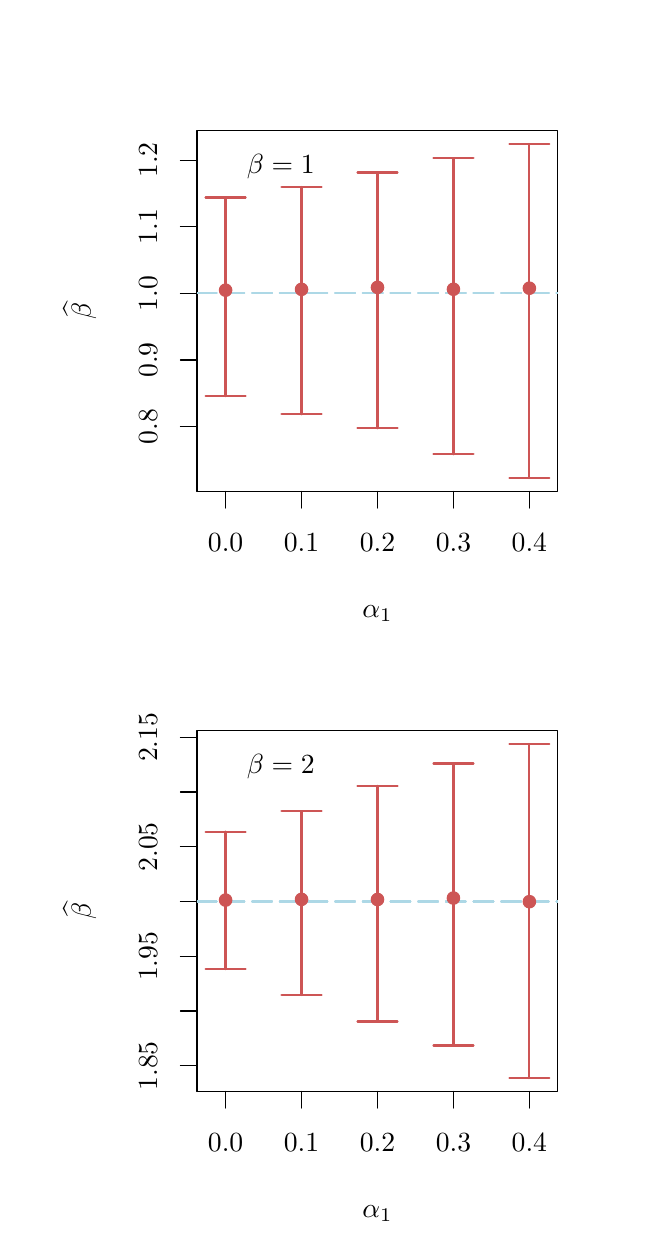
\begin{tikzpicture}[x=1pt,y=1pt]
\definecolor{fillColor}{RGB}{255,255,255}
\path[use as bounding box,fill=fillColor,fill opacity=0.00] (0,0) rectangle (216.81,433.62);
\begin{scope}
\path[clip] ( 61.20,266.01) rectangle (191.61,396.42);
\definecolor{drawColor}{RGB}{255,255,255}
\definecolor{fillColor}{RGB}{255,255,255}

\path[draw=drawColor,line width= 0.4pt,line join=round,line cap=round,fill=fillColor] ( 71.52,338.76) circle (  2.25);

\path[draw=drawColor,line width= 0.4pt,line join=round,line cap=round,fill=fillColor] ( 98.96,339.06) circle (  2.25);

\path[draw=drawColor,line width= 0.4pt,line join=round,line cap=round,fill=fillColor] (126.41,339.77) circle (  2.25);

\path[draw=drawColor,line width= 0.4pt,line join=round,line cap=round,fill=fillColor] (153.85,339.09) circle (  2.25);

\path[draw=drawColor,line width= 0.4pt,line join=round,line cap=round,fill=fillColor] (181.29,339.47) circle (  2.25);
\end{scope}
\begin{scope}
\path[clip] (  0.00,  0.00) rectangle (216.81,433.62);
\definecolor{drawColor}{RGB}{0,0,0}

\path[draw=drawColor,line width= 0.4pt,line join=round,line cap=round] ( 71.52,266.01) -- (181.29,266.01);

\path[draw=drawColor,line width= 0.4pt,line join=round,line cap=round] ( 71.52,266.01) -- ( 71.52,260.01);

\path[draw=drawColor,line width= 0.4pt,line join=round,line cap=round] ( 98.96,266.01) -- ( 98.96,260.01);

\path[draw=drawColor,line width= 0.4pt,line join=round,line cap=round] (126.41,266.01) -- (126.41,260.01);

\path[draw=drawColor,line width= 0.4pt,line join=round,line cap=round] (153.85,266.01) -- (153.85,260.01);

\path[draw=drawColor,line width= 0.4pt,line join=round,line cap=round] (181.29,266.01) -- (181.29,260.01);

\node[text=drawColor,anchor=base,inner sep=0pt, outer sep=0pt, scale=  1.00] at ( 71.52,244.41) {0.0};

\node[text=drawColor,anchor=base,inner sep=0pt, outer sep=0pt, scale=  1.00] at ( 98.96,244.41) {0.1};

\node[text=drawColor,anchor=base,inner sep=0pt, outer sep=0pt, scale=  1.00] at (126.41,244.41) {0.2};

\node[text=drawColor,anchor=base,inner sep=0pt, outer sep=0pt, scale=  1.00] at (153.85,244.41) {0.3};

\node[text=drawColor,anchor=base,inner sep=0pt, outer sep=0pt, scale=  1.00] at (181.29,244.41) {0.4};

\path[draw=drawColor,line width= 0.4pt,line join=round,line cap=round] ( 61.20,289.45) -- ( 61.20,385.76);

\path[draw=drawColor,line width= 0.4pt,line join=round,line cap=round] ( 61.20,289.45) -- ( 55.20,289.45);

\path[draw=drawColor,line width= 0.4pt,line join=round,line cap=round] ( 61.20,313.53) -- ( 55.20,313.53);

\path[draw=drawColor,line width= 0.4pt,line join=round,line cap=round] ( 61.20,337.61) -- ( 55.20,337.61);

\path[draw=drawColor,line width= 0.4pt,line join=round,line cap=round] ( 61.20,361.69) -- ( 55.20,361.69);

\path[draw=drawColor,line width= 0.4pt,line join=round,line cap=round] ( 61.20,385.76) -- ( 55.20,385.76);

\node[text=drawColor,rotate= 90.00,anchor=base,inner sep=0pt, outer sep=0pt, scale=  1.00] at ( 46.80,289.45) {0.8};

\node[text=drawColor,rotate= 90.00,anchor=base,inner sep=0pt, outer sep=0pt, scale=  1.00] at ( 46.80,313.53) {0.9};

\node[text=drawColor,rotate= 90.00,anchor=base,inner sep=0pt, outer sep=0pt, scale=  1.00] at ( 46.80,337.61) {1.0};

\node[text=drawColor,rotate= 90.00,anchor=base,inner sep=0pt, outer sep=0pt, scale=  1.00] at ( 46.80,361.69) {1.1};

\node[text=drawColor,rotate= 90.00,anchor=base,inner sep=0pt, outer sep=0pt, scale=  1.00] at ( 46.80,385.76) {1.2};

\path[draw=drawColor,line width= 0.4pt,line join=round,line cap=round] ( 61.20,266.01) --
	(191.61,266.01) --
	(191.61,396.42) --
	( 61.20,396.42) --
	( 61.20,266.01);
\end{scope}
\begin{scope}
\path[clip] (  0.00,216.81) rectangle (216.81,433.62);
\definecolor{drawColor}{RGB}{0,0,0}

\node[text=drawColor,anchor=base,inner sep=0pt, outer sep=0pt, scale=  1.00] at (126.41,220.41) {$\alpha_1$};

\node[text=drawColor,rotate= 90.00,anchor=base,inner sep=0pt, outer sep=0pt, scale=  1.00] at ( 22.80,331.22) {$\widehat{\beta}$};
\end{scope}
\begin{scope}
\path[clip] ( 61.20,266.01) rectangle (191.61,396.42);
\definecolor{drawColor}{RGB}{0,0,0}

\node[text=drawColor,anchor=base west,inner sep=0pt, outer sep=0pt, scale=  1.00] at ( 79.20,380.98) {$\beta=1$};
\definecolor{drawColor}{RGB}{173,216,230}

\path[draw=drawColor,line width= 0.8pt,dash pattern=on 7pt off 3pt ,line join=round,line cap=round] ( 61.20,337.61) -- (191.61,337.61);

\path[draw=drawColor,line width= 0.8pt,dash pattern=on 7pt off 3pt ,line join=round,line cap=round] ( 61.20,337.61) -- (191.61,337.61);

\path[draw=drawColor,line width= 0.8pt,dash pattern=on 7pt off 3pt ,line join=round,line cap=round] ( 61.20,337.61) -- (191.61,337.61);

\path[draw=drawColor,line width= 0.8pt,dash pattern=on 7pt off 3pt ,line join=round,line cap=round] ( 61.20,337.61) -- (191.61,337.61);

\path[draw=drawColor,line width= 0.8pt,dash pattern=on 7pt off 3pt ,line join=round,line cap=round] ( 61.20,337.61) -- (191.61,337.61);
\definecolor{drawColor}{RGB}{205,85,85}

\path[draw=drawColor,line width= 0.8pt,line join=round,line cap=round] ( 71.52,300.47) -- ( 71.52,372.28);

\path[draw=drawColor,line width= 0.8pt,line join=round,line cap=round] ( 64.29,300.47) --
	( 71.52,300.47) --
	( 78.75,300.47);

\path[draw=drawColor,line width= 0.8pt,line join=round,line cap=round] ( 78.75,372.28) --
	( 71.52,372.28) --
	( 64.29,372.28);

\path[draw=drawColor,line width= 0.8pt,line join=round,line cap=round] ( 98.96,293.91) -- ( 98.96,376.04);

\path[draw=drawColor,line width= 0.8pt,line join=round,line cap=round] ( 91.73,293.91) --
	( 98.96,293.91) --
	(106.19,293.91);

\path[draw=drawColor,line width= 0.8pt,line join=round,line cap=round] (106.19,376.04) --
	( 98.96,376.04) --
	( 91.73,376.04);

\path[draw=drawColor,line width= 0.8pt,line join=round,line cap=round] (126.41,288.86) -- (126.41,381.25);

\path[draw=drawColor,line width= 0.8pt,line join=round,line cap=round] (119.18,288.86) --
	(126.41,288.86) --
	(133.63,288.86);

\path[draw=drawColor,line width= 0.8pt,line join=round,line cap=round] (133.63,381.25) --
	(126.41,381.25) --
	(119.18,381.25);

\path[draw=drawColor,line width= 0.8pt,line join=round,line cap=round] (153.85,279.45) -- (153.85,386.47);

\path[draw=drawColor,line width= 0.8pt,line join=round,line cap=round] (146.62,279.45) --
	(153.85,279.45) --
	(161.08,279.45);

\path[draw=drawColor,line width= 0.8pt,line join=round,line cap=round] (161.08,386.47) --
	(153.85,386.47) --
	(146.62,386.47);

\path[draw=drawColor,line width= 0.8pt,line join=round,line cap=round] (181.29,270.84) -- (181.29,391.59);

\path[draw=drawColor,line width= 0.8pt,line join=round,line cap=round] (174.06,270.84) --
	(181.29,270.84) --
	(188.52,270.84);

\path[draw=drawColor,line width= 0.8pt,line join=round,line cap=round] (188.52,391.59) --
	(181.29,391.59) --
	(174.06,391.59);
\definecolor{fillColor}{RGB}{205,85,85}

\path[draw=drawColor,line width= 0.4pt,line join=round,line cap=round,fill=fillColor] ( 71.52,338.76) circle (  2.25);

\path[draw=drawColor,line width= 0.4pt,line join=round,line cap=round,fill=fillColor] ( 98.96,339.06) circle (  2.25);

\path[draw=drawColor,line width= 0.4pt,line join=round,line cap=round,fill=fillColor] (126.41,339.77) circle (  2.25);

\path[draw=drawColor,line width= 0.4pt,line join=round,line cap=round,fill=fillColor] (153.85,339.09) circle (  2.25);

\path[draw=drawColor,line width= 0.4pt,line join=round,line cap=round,fill=fillColor] (181.29,339.47) circle (  2.25);
\end{scope}
\begin{scope}
\path[clip] ( 61.20, 49.20) rectangle (191.61,179.61);
\definecolor{drawColor}{RGB}{255,255,255}
\definecolor{fillColor}{RGB}{255,255,255}

\path[draw=drawColor,line width= 0.4pt,line join=round,line cap=round,fill=fillColor] ( 71.52,118.37) circle (  2.25);

\path[draw=drawColor,line width= 0.4pt,line join=round,line cap=round,fill=fillColor] ( 98.96,118.63) circle (  2.25);

\path[draw=drawColor,line width= 0.4pt,line join=round,line cap=round,fill=fillColor] (126.41,118.58) circle (  2.25);

\path[draw=drawColor,line width= 0.4pt,line join=round,line cap=round,fill=fillColor] (153.85,119.11) circle (  2.25);

\path[draw=drawColor,line width= 0.4pt,line join=round,line cap=round,fill=fillColor] (181.29,117.80) circle (  2.25);
\end{scope}
\begin{scope}
\path[clip] (  0.00,  0.00) rectangle (216.81,433.62);
\definecolor{drawColor}{RGB}{0,0,0}

\path[draw=drawColor,line width= 0.4pt,line join=round,line cap=round] ( 71.52, 49.20) -- (181.29, 49.20);

\path[draw=drawColor,line width= 0.4pt,line join=round,line cap=round] ( 71.52, 49.20) -- ( 71.52, 43.20);

\path[draw=drawColor,line width= 0.4pt,line join=round,line cap=round] ( 98.96, 49.20) -- ( 98.96, 43.20);

\path[draw=drawColor,line width= 0.4pt,line join=round,line cap=round] (126.41, 49.20) -- (126.41, 43.20);

\path[draw=drawColor,line width= 0.4pt,line join=round,line cap=round] (153.85, 49.20) -- (153.85, 43.20);

\path[draw=drawColor,line width= 0.4pt,line join=round,line cap=round] (181.29, 49.20) -- (181.29, 43.20);

\node[text=drawColor,anchor=base,inner sep=0pt, outer sep=0pt, scale=  1.00] at ( 71.52, 27.60) {0.0};

\node[text=drawColor,anchor=base,inner sep=0pt, outer sep=0pt, scale=  1.00] at ( 98.96, 27.60) {0.1};

\node[text=drawColor,anchor=base,inner sep=0pt, outer sep=0pt, scale=  1.00] at (126.41, 27.60) {0.2};

\node[text=drawColor,anchor=base,inner sep=0pt, outer sep=0pt, scale=  1.00] at (153.85, 27.60) {0.3};

\node[text=drawColor,anchor=base,inner sep=0pt, outer sep=0pt, scale=  1.00] at (181.29, 27.60) {0.4};

\path[draw=drawColor,line width= 0.4pt,line join=round,line cap=round] ( 61.20, 58.49) -- ( 61.20,177.20);

\path[draw=drawColor,line width= 0.4pt,line join=round,line cap=round] ( 61.20, 58.49) -- ( 55.20, 58.49);

\path[draw=drawColor,line width= 0.4pt,line join=round,line cap=round] ( 61.20, 78.28) -- ( 55.20, 78.28);

\path[draw=drawColor,line width= 0.4pt,line join=round,line cap=round] ( 61.20, 98.06) -- ( 55.20, 98.06);

\path[draw=drawColor,line width= 0.4pt,line join=round,line cap=round] ( 61.20,117.85) -- ( 55.20,117.85);

\path[draw=drawColor,line width= 0.4pt,line join=round,line cap=round] ( 61.20,137.63) -- ( 55.20,137.63);

\path[draw=drawColor,line width= 0.4pt,line join=round,line cap=round] ( 61.20,157.41) -- ( 55.20,157.41);

\path[draw=drawColor,line width= 0.4pt,line join=round,line cap=round] ( 61.20,177.20) -- ( 55.20,177.20);

\node[text=drawColor,rotate= 90.00,anchor=base,inner sep=0pt, outer sep=0pt, scale=  1.00] at ( 46.80, 58.49) {1.85};

\node[text=drawColor,rotate= 90.00,anchor=base,inner sep=0pt, outer sep=0pt, scale=  1.00] at ( 46.80, 98.06) {1.95};

\node[text=drawColor,rotate= 90.00,anchor=base,inner sep=0pt, outer sep=0pt, scale=  1.00] at ( 46.80,137.63) {2.05};

\node[text=drawColor,rotate= 90.00,anchor=base,inner sep=0pt, outer sep=0pt, scale=  1.00] at ( 46.80,177.20) {2.15};

\path[draw=drawColor,line width= 0.4pt,line join=round,line cap=round] ( 61.20, 49.20) --
	(191.61, 49.20) --
	(191.61,179.61) --
	( 61.20,179.61) --
	( 61.20, 49.20);
\end{scope}
\begin{scope}
\path[clip] (  0.00,  0.00) rectangle (216.81,216.81);
\definecolor{drawColor}{RGB}{0,0,0}

\node[text=drawColor,anchor=base,inner sep=0pt, outer sep=0pt, scale=  1.00] at (126.41,  3.60) {$\alpha_1$};

\node[text=drawColor,rotate= 90.00,anchor=base,inner sep=0pt, outer sep=0pt, scale=  1.00] at ( 22.80,114.41) {$\widehat{\beta}$};
\end{scope}
\begin{scope}
\path[clip] ( 61.20, 49.20) rectangle (191.61,179.61);
\definecolor{drawColor}{RGB}{0,0,0}

\node[text=drawColor,anchor=base west,inner sep=0pt, outer sep=0pt, scale=  1.00] at ( 79.20,164.17) {$\beta=2$};
\definecolor{drawColor}{RGB}{173,216,230}

\path[draw=drawColor,line width= 0.8pt,dash pattern=on 7pt off 3pt ,line join=round,line cap=round] ( 61.20,117.85) -- (191.61,117.85);

\path[draw=drawColor,line width= 0.8pt,dash pattern=on 7pt off 3pt ,line join=round,line cap=round] ( 61.20,117.85) -- (191.61,117.85);

\path[draw=drawColor,line width= 0.8pt,dash pattern=on 7pt off 3pt ,line join=round,line cap=round] ( 61.20,117.85) -- (191.61,117.85);

\path[draw=drawColor,line width= 0.8pt,dash pattern=on 7pt off 3pt ,line join=round,line cap=round] ( 61.20,117.85) -- (191.61,117.85);

\path[draw=drawColor,line width= 0.8pt,dash pattern=on 7pt off 3pt ,line join=round,line cap=round] ( 61.20,117.85) -- (191.61,117.85);
\definecolor{drawColor}{RGB}{205,85,85}

\path[draw=drawColor,line width= 0.8pt,line join=round,line cap=round] ( 71.52, 93.44) -- ( 71.52,143.11);

\path[draw=drawColor,line width= 0.8pt,line join=round,line cap=round] ( 64.29, 93.44) --
	( 71.52, 93.44) --
	( 78.75, 93.44);

\path[draw=drawColor,line width= 0.8pt,line join=round,line cap=round] ( 78.75,143.11) --
	( 71.52,143.11) --
	( 64.29,143.11);

\path[draw=drawColor,line width= 0.8pt,line join=round,line cap=round] ( 98.96, 84.05) -- ( 98.96,150.43);

\path[draw=drawColor,line width= 0.8pt,line join=round,line cap=round] ( 91.73, 84.05) --
	( 98.96, 84.05) --
	(106.19, 84.05);

\path[draw=drawColor,line width= 0.8pt,line join=round,line cap=round] (106.19,150.43) --
	( 98.96,150.43) --
	( 91.73,150.43);

\path[draw=drawColor,line width= 0.8pt,line join=round,line cap=round] (126.41, 74.47) -- (126.41,159.63);

\path[draw=drawColor,line width= 0.8pt,line join=round,line cap=round] (119.18, 74.47) --
	(126.41, 74.47) --
	(133.63, 74.47);

\path[draw=drawColor,line width= 0.8pt,line join=round,line cap=round] (133.63,159.63) --
	(126.41,159.63) --
	(119.18,159.63);

\path[draw=drawColor,line width= 0.8pt,line join=round,line cap=round] (153.85, 65.82) -- (153.85,167.70);

\path[draw=drawColor,line width= 0.8pt,line join=round,line cap=round] (146.62, 65.82) --
	(153.85, 65.82) --
	(161.08, 65.82);

\path[draw=drawColor,line width= 0.8pt,line join=round,line cap=round] (161.08,167.70) --
	(153.85,167.70) --
	(146.62,167.70);

\path[draw=drawColor,line width= 0.8pt,line join=round,line cap=round] (181.29, 54.03) -- (181.29,174.78);

\path[draw=drawColor,line width= 0.8pt,line join=round,line cap=round] (174.06, 54.03) --
	(181.29, 54.03) --
	(188.52, 54.03);

\path[draw=drawColor,line width= 0.8pt,line join=round,line cap=round] (188.52,174.78) --
	(181.29,174.78) --
	(174.06,174.78);
\definecolor{fillColor}{RGB}{205,85,85}

\path[draw=drawColor,line width= 0.4pt,line join=round,line cap=round,fill=fillColor] ( 71.52,118.37) circle (  2.25);

\path[draw=drawColor,line width= 0.4pt,line join=round,line cap=round,fill=fillColor] ( 98.96,118.63) circle (  2.25);

\path[draw=drawColor,line width= 0.4pt,line join=round,line cap=round,fill=fillColor] (126.41,118.58) circle (  2.25);

\path[draw=drawColor,line width= 0.4pt,line join=round,line cap=round,fill=fillColor] (153.85,119.11) circle (  2.25);

\path[draw=drawColor,line width= 0.4pt,line join=round,line cap=round,fill=fillColor] (181.29,117.80) circle (  2.25);
\end{scope}
\end{tikzpicture}
